\documentclass{report}
\usepackage[spanish]{babel}
\usepackage[utf8]{inputenc}
\usepackage{graphicx, longtable, float, titlesec, hyperref}

\hypersetup{
    hidelinks = true
}

\titleformat{\chapter}[display]
  {\normalfont\bfseries}{}{0pt}{\Huge}

\begin{document}
    \begin{titlepage}
        \centering
        
\includegraphics[width=0.6\textwidth]{./img/miscelanio/logo.jpg}\\
        \vspace{1cm}
        \LARGE Sistemas de Gestión de Seguridad de Sistemas de Información\\
        \vspace{0.5cm}
        \Large Ingeniería Informática de Gestión y Sistemas de Información\\
        \vspace{3cm}
        \Huge Sistema Web\\
        \vspace{2.5cm}
        \Large Autores:\\
        \vspace{0.2cm}
        \large Xabier Gabiña\\
        \large Ainhize Martinez\\
        \large Marcos Martín\\
        \vfill
        \today
    \end{titlepage}
    \tableofcontents
    \chapter{Introduccion}
    \chapter{Primera auditoria}
        La idea de esta auditoria es la de encontrar los fallos de seguridad que tiene nuestro sistema web para en el posterior capitulo de este documento comentarlos y solucionarlos.\\
        \section{ZAP}
        Para empezar con la primera auditoria ejecutaremos el proxy ZAP como se nos ha propuesto en clase.
        Al ejecutarla en nuestra pagina web nos encontramos con el siguiente listado de errores:
        \begin{figure}[H]
            \centering
            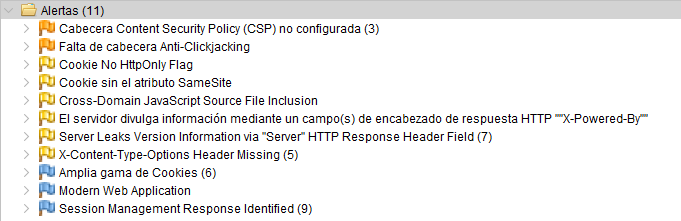
\includegraphics[width=\textwidth]{./img/audit1/zap1.png}
            \caption{Listado de errores de la primera auditoria}
        \end{figure}
        Como podemos ver en la imagen, tenemos un total de 11 errores, los cuales iremos comentando uno a uno en los siguientes apartados y solucionando.
        \section{sqlmap}
        \section{nmap}
        \section{Metaexploit}
    \chapter{Vulnerabilidades}
        \section{Rotura de control de acceso}
            La rotura de control de acceso es una vulnerabilidad que permite a un atacante acceder a recursos restringidos o privilegiados, ya sea por un error en la implementación de la autenticación y autorización o por un error en la lógica de control de acceso.
            Dentro de nuestro sistema tenemos varios fallos de rotura de control y ahora hablaremos de ellas y de como las hemos solucionado.
            \subsection{Control de acceso}
                \subsubsection{Descripción}
                    En nuestro sistema, un usuario puede modificar sus datos personales, pero también puede modificar los datos de otros usuarios. 
                    Esto es un fallo de rotura de control de acceso ya que un usuario no debería poder modificar los datos de otro usuario.
                \subsubsection{PoC}
                    Pongamos en el ejemplo que tenemos dos usuarios, Admin y Xabier con sus repectivas IDs
                    \begin{figure}[H]
                        \centering
                        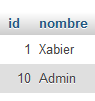
\includegraphics[width=0.2\textwidth]{./img/vulnerabilidades/3.1.1.1.png}
                        \caption{Datos de Usuarios}
                    \end{figure}
                    Si desde inspeccionar elementos hacemos click sobre el boton 'Perfil' este nos mostrara el link el cual se ve asi:
                    \begin{figure}[H]
                        \centering
                        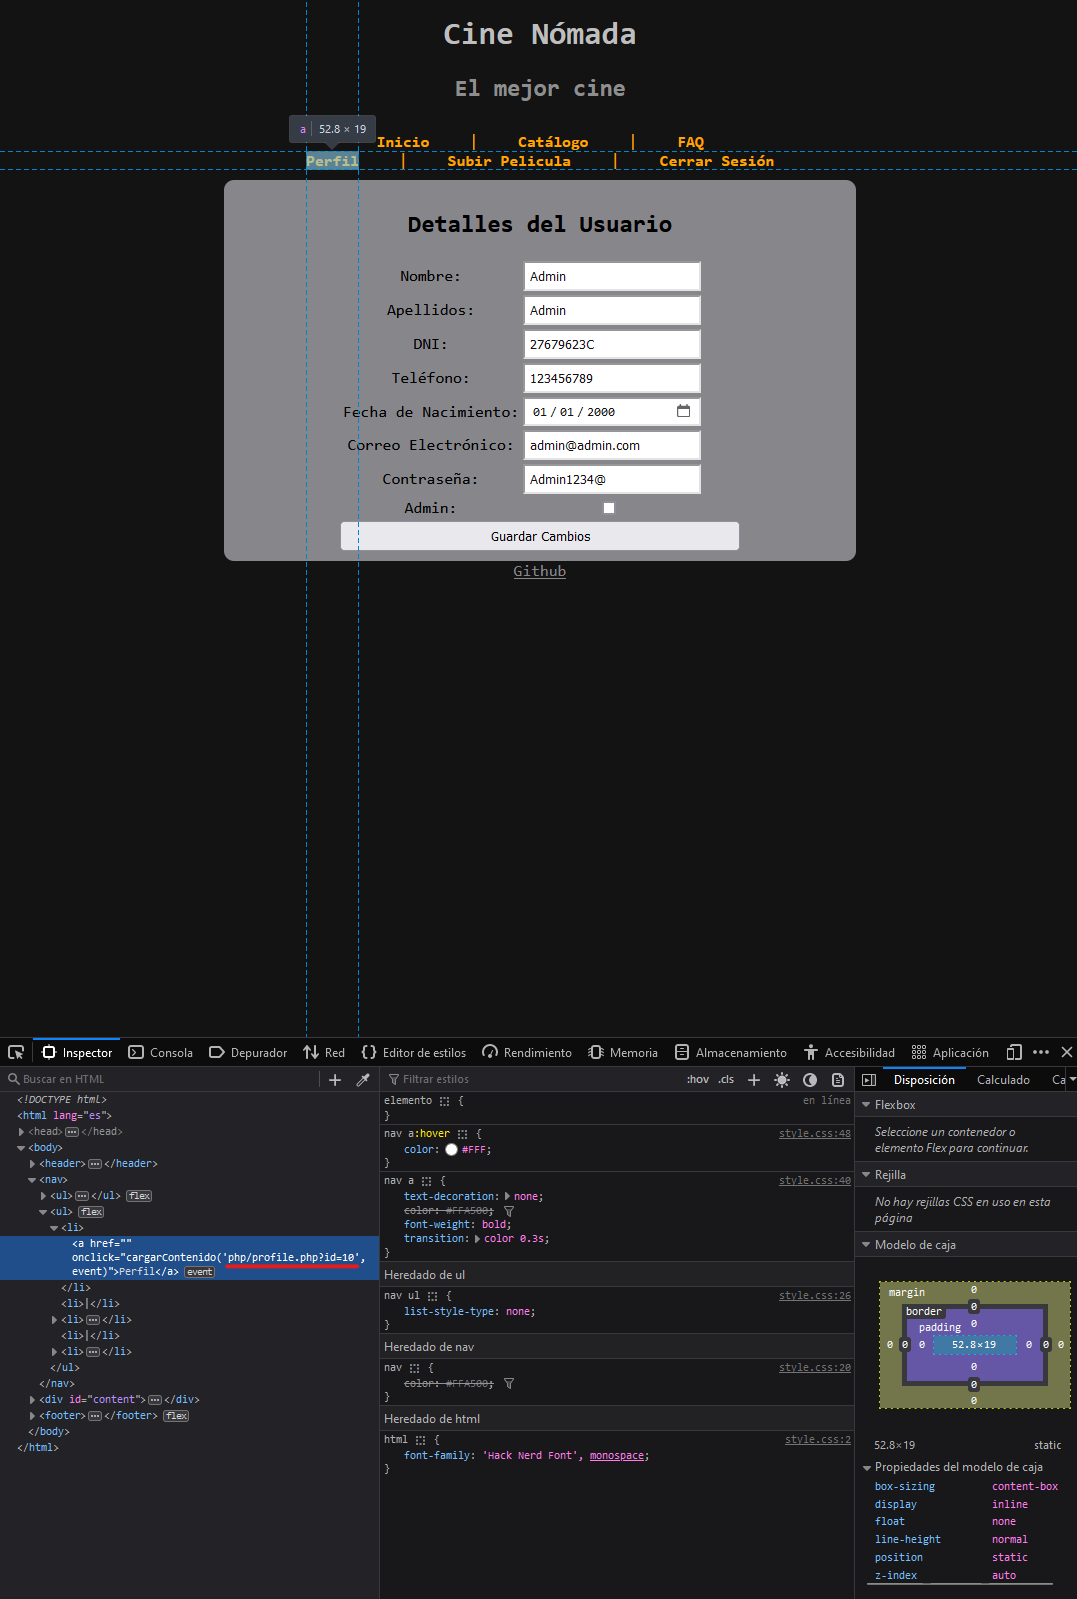
\includegraphics[width=0.8\textwidth]{./img/vulnerabilidades/3.1.1.2.png}
                        \caption{Perfil de Admin}
                    \end{figure}
                    Si alteramos el valor de ?id=X por en este caso la id de Xabier (La ID 1) podemos acceder a sus datos
                    \begin{figure}[H]
                        \centering
                        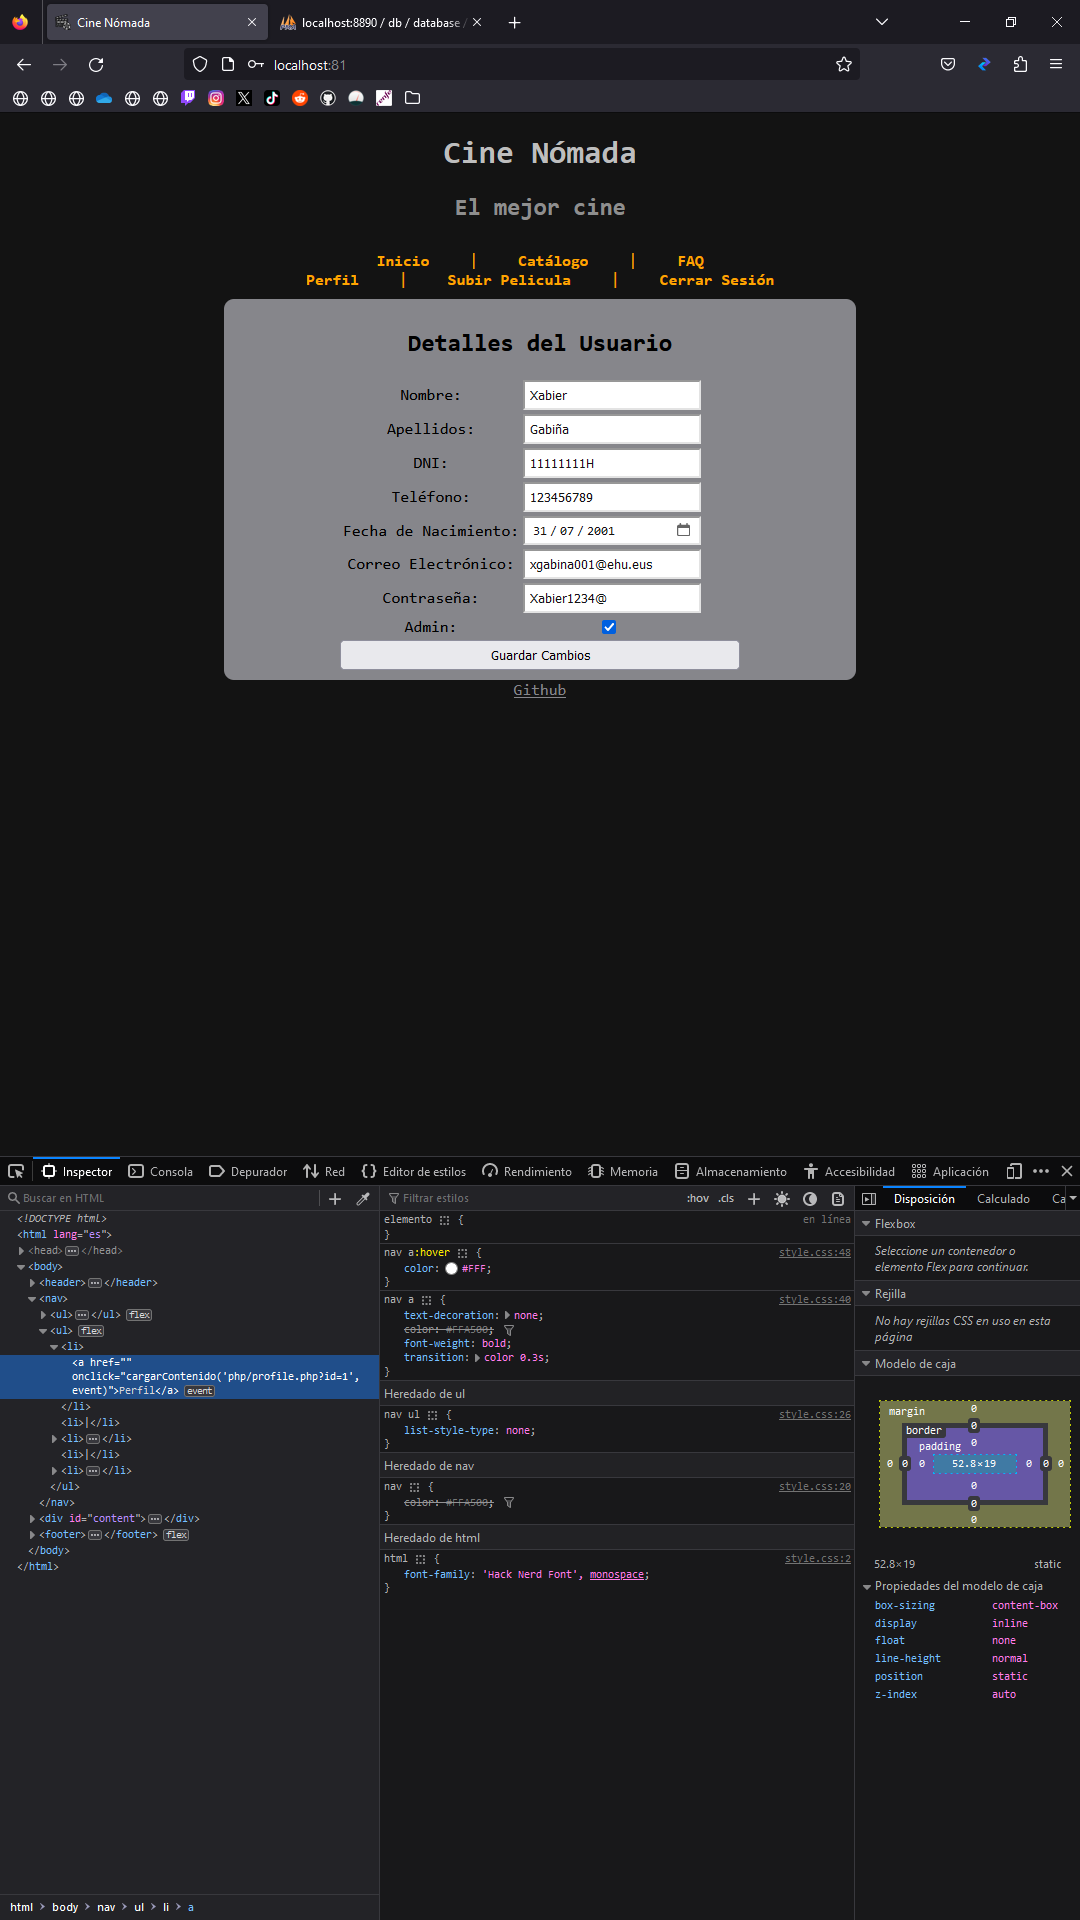
\includegraphics[width=\textwidth]{./img/vulnerabilidades/3.1.1.3.png}
                        \caption{Perfil de Xabier}
                    \end{figure}
                \subsubsection{Solución}
                    Para solucionar este problema, hemos añadido una comprobación en el código que comprueba que el usuario que está intentando modificar los datos es el mismo que el usuario que está logueado en el sistema.
                    \begin{figure}[H]
                        \centering
                        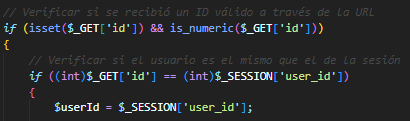
\includegraphics[width=\textwidth]{./img/vulnerabilidades/3.1.1.4.png}
                        \caption{Comprobación de usuario}
                    \end{figure}
                    Esta misma error tambien ha sido corregido en el catalogo.
            \clearpage       
        \section{Fallos criptográficos}
            \subsection{Cifrado de extremo a extremo}
                \subsubsection{Descripción}
                    En nuestro sistema, no se fuerza el uso de HTTPS, lo que permite que un atacante pueda interceptar el trafico de la pagina y obtener información sensible de los usuarios.
                \subsubsection{Solución}
                    Para solucionar este problema configuraremos nuestro servidor para que cifre y rediriga todo el trafico a HTTPS.
                    
                    Creamos un certificado SSL autofirmado dentro del Dockerfile.
                    
                    Creamos una regla para redirigir el trafico entrante del puerto 80 al puerto 443.
                    \begin{figure}[H]
                        \centering
                        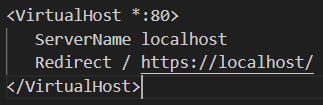
\includegraphics[width=\textwidth]{./img/vulnerabilidades/3.2.1.1.png}
                        \caption{Redireccion de trafico}
                    \end{figure}
                    
                    Tambien debemos decir al puerto 443 que use el certificado SSL que hemos creado.
                    \begin{figure}[H]
                        \centering
                        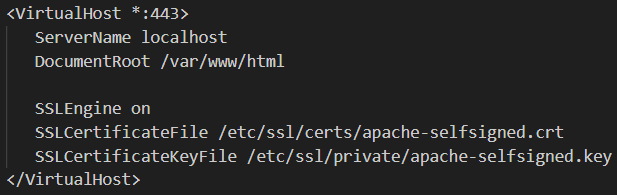
\includegraphics[width=\textwidth]{./img/vulnerabilidades/3.2.1.2.png}
                        \caption{Certificado SSL}
                    \end{figure}
            \clearpage
            \subsection{Almacenar informacion sensible}
            \clearpage
            \subsection{Almacenamiento de contraseñas}
                \subsubsection{Descripción}
                    En nuestro sistema, no se almacenan las contraseñas de los usuarios de forma segura, lo que permite que un atacante pueda obtener las contraseñas de los usuarios.
                \subsubsection{PoC}
                    Si un atacante consigue acceso a la base de datos, puede obtener las contraseñas de los usuarios en texto plano.
                    \begin{figure}[H]
                        \centering
                        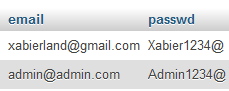
\includegraphics[width=\textwidth]{./img/vulnerabilidades/3.2.3.1.png}
                        \caption{Contraseñas en texto plano}
                    \end{figure}
                \subsubsection{Solución}
                    Para solucionar este problema de la mejor forma posible debemos tener tres puntos bien definidos:
                    \begin{enumerate}
                        \item Cofigurar el factor de costo apropiado
                        \begin{itemize}
                            \item El factor de costo (work factor) en bcrypt determina el número de iteraciones utilizadas en el cálculo del hash. Un valor mayor implica una contraseña más segura, pero también requiere más tiempo para calcular el hash. Un valor razonable es 12 o más, dependiendo del hardware y las necesidades de rendimiento.
                        \end{itemize}
                        \item Usar un algoritmo de cifrado seguro.
                        \begin{itemize}
                            \item En nuestro caso usaremos BCrypt. CRYPT\_BLOWFISH se usa para crear el hash. Producirá un hash estándar compatible con crypt() utilizando el identificador \texttt{"\$2y\$"}. El resultado siempre será un string de 60 caracteres, o false en caso de error.
                        \end{itemize}
                        \item Generar un semilla aleatoria para cada usuario.
                        \begin{itemize}
                            \item BCrypt ya gestiona las semillas de forma automatica y en el manual de PHP no recomiendan su uso de otra manera. Mas informacion en \url{https://www.php.net/manual/es/function.password-hash.php}
                        \end{itemize}
                    \end{enumerate}
                    \begin{figure}[H]
                        \centering
                        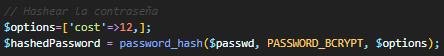
\includegraphics[width=\textwidth]{./img/vulnerabilidades/3.2.3.2.png}
                        \caption{Contraseñas encriptadas}
                    \end{figure}
            \clearpage
            \subsection{Configuracion erronea de las Cookies}
                \subsubsection{Descripción}
                    La configuración errónea de las cookies se refiere a la práctica de establecer parámetros o atributos de las cookies de manera inadecuada, lo que puede tener consecuencias negativas en términos de seguridad, privacidad y funcionalidad en una aplicación web.                
                \subsubsection{Solución}
                    Para solucionar este problema, hemos añadido una configuración segura a las cookies de nuestro sitio web.
                    \begin{figure}[H]
                        \centering
                        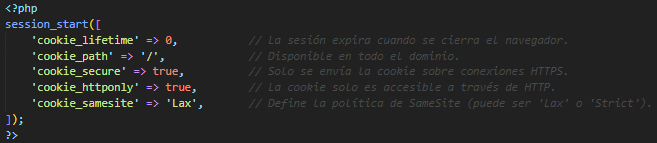
\includegraphics[width=\textwidth]{./img/vulnerabilidades/3.2.4.1.png}
                        \caption{Configuración de las cookies}
                    \end{figure}
            \clearpage
        \section{Inyección}
            \subsection{Procesado de consultar SQL}
                \subsubsection{Descripción}
                    En nuestro sistema, no se procesan correctamente las consultas SQL, lo que permite que un atacante pueda obtener información sensible de los usuarios.
                \subsubsection{PoC}
                \subsubsection{Solución}
                    Para solucionar este problema, hemos modificado el codigo que procesa las consultas SQL para que no se puedan inyectar consultas SQL.
                    \begin{figure}[H]
                        \centering
                        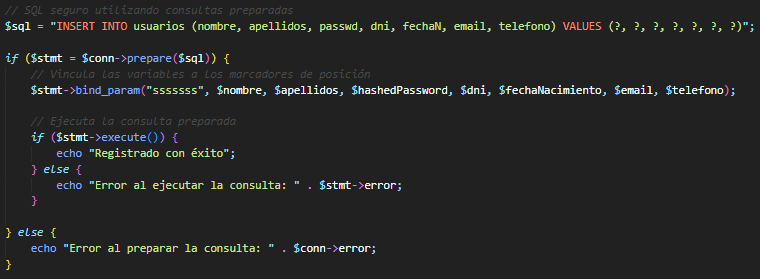
\includegraphics[width=\textwidth]{./img/vulnerabilidades/3.3.1.1.png}
                        \caption{Parametrizar consulta SQL}
                    \end{figure}
            \clearpage
        \section{Diseño inseguro}
            \subsection{Auditorias de seguridad}
                \subsubsection{Descripción}
                    Una auditoría de seguridad es un proceso sistemático de evaluación y revisión de sistemas, redes, aplicaciones o entornos tecnológicos con el propósito de identificar vulnerabilidades, debilidades y riesgos de seguridad. El objetivo principal de una auditoría de seguridad es garantizar que los controles de seguridad estén implementados adecuadamente y cumplan con los estándares de seguridad, y proporcionar recomendaciones para mejorar la protección de activos y datos contra amenazas y ataques cibernéticos.
                \subsubsection{Solución}
                    La solucion a este problema es realizar una auditoria de seguridad de forma periodica para detectar posibles fallos de seguridad. 
            \clearpage
            \subsection{Reutilizacion de codigos seguros}
                \subsubsection{Descripción}
                    La reutilización de código seguro se refiere a la práctica de aprovechar componentes de software previamente probados y seguros en lugar de escribir código desde cero. Esto no solo puede acelerar el desarrollo de software, sino que también puede reducir el riesgo de introducir vulnerabilidades de seguridad.
                \subsubsection{Solución}
                    En nuestro proyecto se han implementado estas practicas mediante la reutilización del archivo validar.js en el que se encuentran las funciones de validación de todos los formularios de nuestro sitio web.
            \clearpage
        \section{Configuración de seguridad insuficiente}
            \subsection{Entornos de desarrollo}
                \subsubsection{Descripción}
                    GitHub
                \subsubsection{Solución}
            \clearpage
            \subsection{Plataforma minima}
                \subsubsection{Descripción}
                \subsubsection{Solución}
            \clearpage
            \subsection{Despliegue seguro}
                \subsubsection{Descripción}
                    Es importante que a la hora de montar nuestro servidor web no haya archivos que puedan ser accesibles desde el exterior y que puedan contener informacion sensible como contraseñas. Esto a nosotros nos ocurre en el docker-compose.yml
                \subsubsection{Solución}
                    Hemos creado un .env donde se almacenan las contraseñas y demas informacion sensible y hemos añadido el archivo al .gitignore para que no se suba al repositorio.
            \clearpage
            \subsection{Cabeceras CSP}
                \subsubsection{Descripción}
                    Las cabeceras CSP son una medida de seguridad utilizada en la programación web para mitigar los riesgos asociados con ataques de Cross-Site Scripting (XSS) y otros tipos de ataques de inyección de código malicioso en páginas web.
                \subsubsection{Solución}
                    Para solucionar este problema, hemos añadido una cabecera 'Content-Security-Policy' con los siguientes valores:
            \clearpage
            \subsection{Cabeceras HSTS}
                \subsubsection{Descripción}
                    Las cabeceras HSTS (HTTP Strict Transport Security) son una medida de seguridad utilizada en la programación web para garantizar que las comunicaciones entre un navegador web y un sitio web se realicen a través de una conexión segura y encriptada utilizando el protocolo HTTPS (HTTP Secure). HSTS ayuda a prevenir ataques de tipo man-in-the-middle (MitM) que podrían exponer datos sensibles o comprometer la seguridad de la comunicación.
                \subsubsection{Solución}
                    Para solucionar este problema, hemos añadido una cabecera 'Strict-Transport-Security' con los siguientes valores:
            \clearpage
            \subsection{Cabeceras X-XSS-Protection}
                \subsubsection{Descripción}
                Las cabeceras "X-XSS-Protection" son una medida de seguridad utilizada en la programación web para ayudar a prevenir ataques de tipo Cross-Site Scripting (XSS). Los ataques XSS ocurren cuando un atacante inyecta código JavaScript malicioso en una página web, que luego se ejecuta en el navegador de un usuario sin su conocimiento. Estas cabeceras se utilizan para controlar y mitigar estos ataques.
                \subsubsection{Solución}
                    Para solucionar este problema, hemos añadido una cabecera 'X-XSS-Protection' con los siguientes valores:
            \clearpage
            \subsection{Cabeceras X-Content-Type-Options}
                \subsubsection{Descripción}
                Las cabeceras "X-Content-Type-Options" son una medida de seguridad utilizada en la programación web para mitigar ciertos tipos de ataques, como ataques de tipo MIME-sniffing. Estas cabeceras se utilizan para controlar cómo el navegador web interpreta y muestra el contenido de una página web.
                \subsubsection{Solución}
                    Para solucionar este problema, hemos añadido una cabecera 'X-Content-Type-Options' con los siguientes valores:
                    \begin{figure}[H]
                        \centering
                        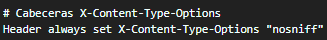
\includegraphics[width=0.7\textwidth]{./img/vulnerabilidades/3.5.7.1.png}
                        \caption{Cabecera X-Content-Type-Options}
                    \end{figure}
            \clearpage
            \subsection{Cabeceras X-Frame-Options}
                \subsubsection{Descripción}
                    Las cabeceras "X-Frame-Options" son una medida de seguridad utilizada en la programación web para controlar si una página web puede ser incrustada o mostrada dentro de un marco (frame) de otro sitio web. Estas cabeceras se utilizan para prevenir ataques de clickjacking, en los cuales un atacante puede ocultar contenido malicioso detrás de una página legítima y engañar a los usuarios para que hagan clic en elementos sin su consentimiento.
                \subsubsection{Solución}
                    Para solucionar este problema, hemos añadido una cabecera 'X-Frame-Options' con los siguientes valores:
                    \begin{figure}[H]
                        \centering
                        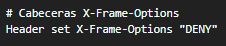
\includegraphics[width=0.7\textwidth]{./img/vulnerabilidades/3.5.8.1.png}
                        \caption{Cabecera X-Frame-Options}
                    \end{figure}
            \clearpage
            \subsection{Cabeceras Cache-Control}
                \subsubsection{Descripción}
                    Las cabeceras 'Cache-Control' son utilizadas en las respuestas HTTP enviadas por un servidor web para controlar cómo los recursos web deben ser almacenados en la memoria caché del navegador o en servidores intermedios (como proxies) y cómo se deben comportar en términos de almacenamiento y actualización. Estas cabeceras son fundamentales para gestionar la eficiencia de la carga de páginas web, la seguridad y la privacidad.
                \subsubsection{Solución}
                    Para solucionar este problema crearemos una cabecera 'Cache-Control' con el valor 'no-store' para que el navegador no almacene en cache la pagina.
                    \begin{figure}[H]
                        \centering
                        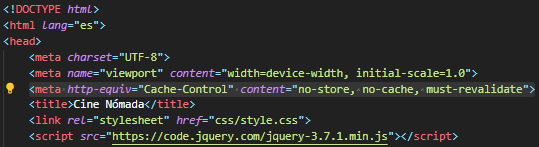
\includegraphics[width=\textwidth]{./img/vulnerabilidades/3.5.9.1.png}
                        \caption{Cabecera Cache-Control}
                    \end{figure}
            \clearpage
            \subsection{Configuracion PHP}
                \subsubsection{Descripción}
                    Cuando usamos PHP en un servidor web es importante el configurarlo de forma segura para evitar que se filtre informacion que pueda ayudar a los atacantes a encontrar una vulnerabilidad en nuestro sistema.
                \subsubsection{Solución}
                    Hemos ocultado la version de PHP en las peticiones a nuestro servidor para evitar que un atacante pueda usar esta informacion para encontrar una vulnerabilidad en nuestro sistema. Para ello hemos creado el php.ini
                    \begin{figure}[H]
                        \centering
                        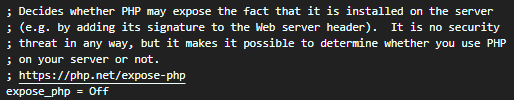
\includegraphics[width=\textwidth]{./img/vulnerabilidades/3.5.10.1.png}
                        \caption{Ocultar version de PHP}
                    \end{figure}
            \clearpage
            \subsection{Configuracion Apache}
                \subsubsection{Descripción}
                    Al igual que con PHP en el punto anterior es importante configurar Apache para que muestre la minima informacion al exterior.
                \subsubsection{Solución}
                    Para ello, al igual que con PHP, hemos ocultado las versiones del servidor para evitar en la medida de lo posible que el atacante encuntre vulnerabilidad en nuestro servidor. Para ello hemos editado el apache2.conf
                    \begin{figure}[H]
                        \centering
                        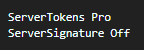
\includegraphics[width=0.7\textwidth]{./img/vulnerabilidades/3.5.11.1.png}
                        \caption{Ocultar version de Apache}
                    \end{figure}
            \clearpage
        \section{Componentes vulnerables y obsoletos}
            \subsection{Control de versiones de los componentes}
                \subsubsection{Descripción}
                    Es crítico mantener actualizados los sistemas operativos y el software de seguridad con las últimas actualizaciones y parches de seguridad.
                \subsubsection{Solución}
                    Para solucionar este problema, hemos actualizado todos los componentes a sus ultimas versiones.
                    \begin{itemize}
                        \item PHP 7.2.2 → 8.2
                        \item MariaDB 10.8.2 → 11.1.2
                        \item phpMyAdmin ya estaba en la ultima version.
                        \item jQuery 3.6.0 → 3.7.1
                    \end{itemize}
            \clearpage
        \section{Fallos de identificación y autenticación}
            \subsection{Autenticacion de dos factores}
            \clearpage
            \subsection{Contraseñas debiles o por defecto}
            \clearpage
            \subsection{Invalidacion de sesiones}
                    \subsubsection{Descripción}
            \clearpage
        \section{Fallos en la integridad de datos y software}
            \subsection{Firmas digitales}
            \clearpage
            \subsection{Bibliotecas y dependencias confiables}
            \clearpage
            \subsection{Uso de herramientas de analisis}
            \clearpage
        \section{Fallos en la monitorizacion de la seguridad}
            \subsection{Configuracion de logs del sistema}
            \clearpage
            \subsection{Implementacion de un log}
            \clearpage
        \section{Falsificacion de Solicitud del Lado del Servidor (SSRF)}
            \subsection{Control del trafico}
               Wireshark/tcpdump
            \clearpage
            \subsection{Validacion de accesos}
                Snort
            \clearpage
            \subsection{Asegurar el codigo}
                GitHub
            \clearpage
        \section{Problemas de calidad de codigo}
            \subsection{Revision de calidad del codigo}
            \clearpage
        \section{Problemas de denegacion de servicios}
            \subsection{Pruebas de rendimiento}
            \clearpage
    \chapter{Segunda auditoria}
        \section{ZAP}
        \section{sqlmap}
        \section{nmap}
        \section{Metaexploit}
    \chapter{Conclusiones}
    \chapter{Bibliografia}
        \begin{itemize}
            \item OWASP. (2021). Informe de Vulnerabilidades. OWASP. \url{https://owasp.org/www-project-top-ten/}
            \item GPT-3.5. (2023). Respuestas a preguntas varias. OpenAI. \url{https://www.openai.com/}
            \item GitHub Copilot. (2022). Autocompletado. GitHub. \url{https://github.com/features/copilot}
        \end{itemize}
\end{document}